\begin{figure}[t]
    \centering
    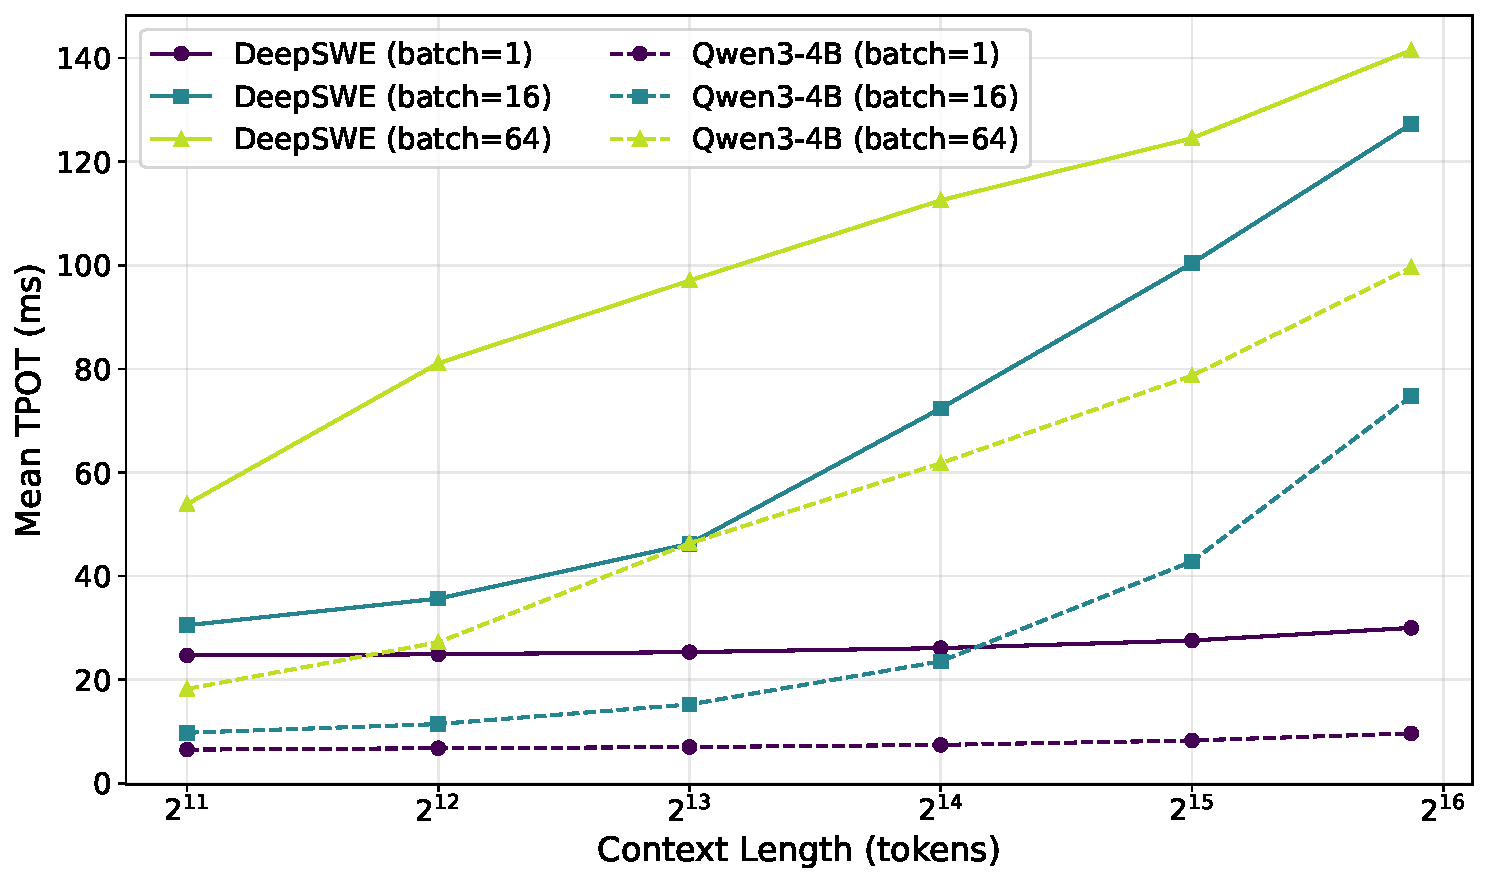
\includegraphics[width=0.96\linewidth]{figs/multi_model_tpot_vs_context_length.pdf}
    \caption{TPOT for two models on various context lengths and batch sizes. DeepSWE is a dense model with $32$B parameters.}
    \label{fig:profile}
    \vspace{-5mm}
\end{figure}
\begin{figure*}[t]
    \centering
    \begin{subfigure}{0.32\textwidth}
        \centering
        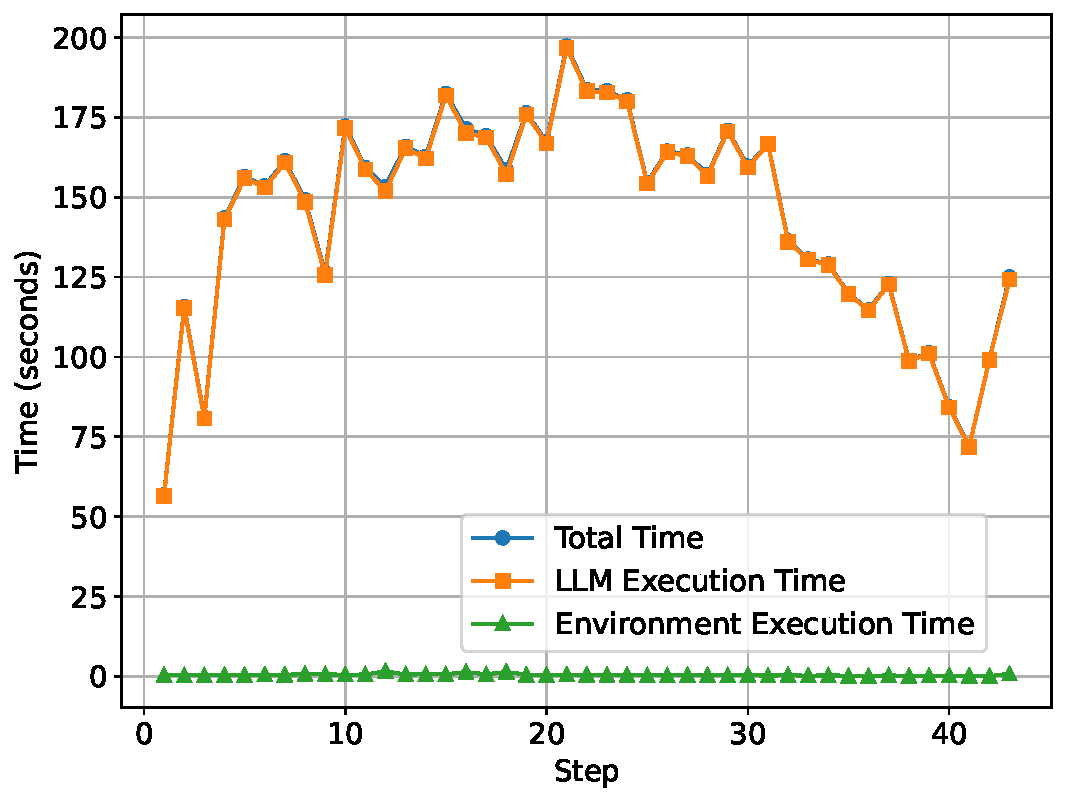
\includegraphics[width=\linewidth]{figs/full_context_time_decomposition.pdf}
        % \caption{AlfWorld}
        \label{fig:success-env1}
    \end{subfigure}
    \hfill
    \begin{subfigure}{0.32\textwidth}
        \centering
        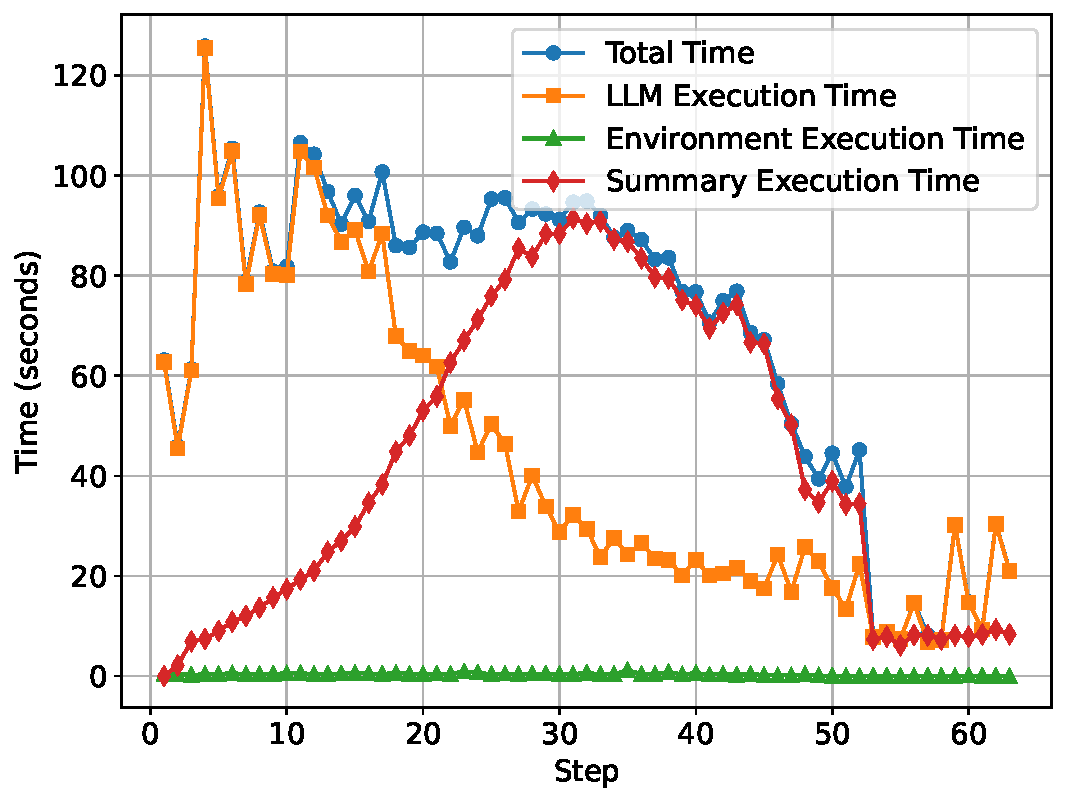
\includegraphics[width=\linewidth]{figs/comem_time_decomposition.pdf}
        % \caption{Webshop}
        \label{fig:success-env2}
    \end{subfigure}
    \hfill
    \begin{subfigure}{0.32\textwidth}
        \centering
        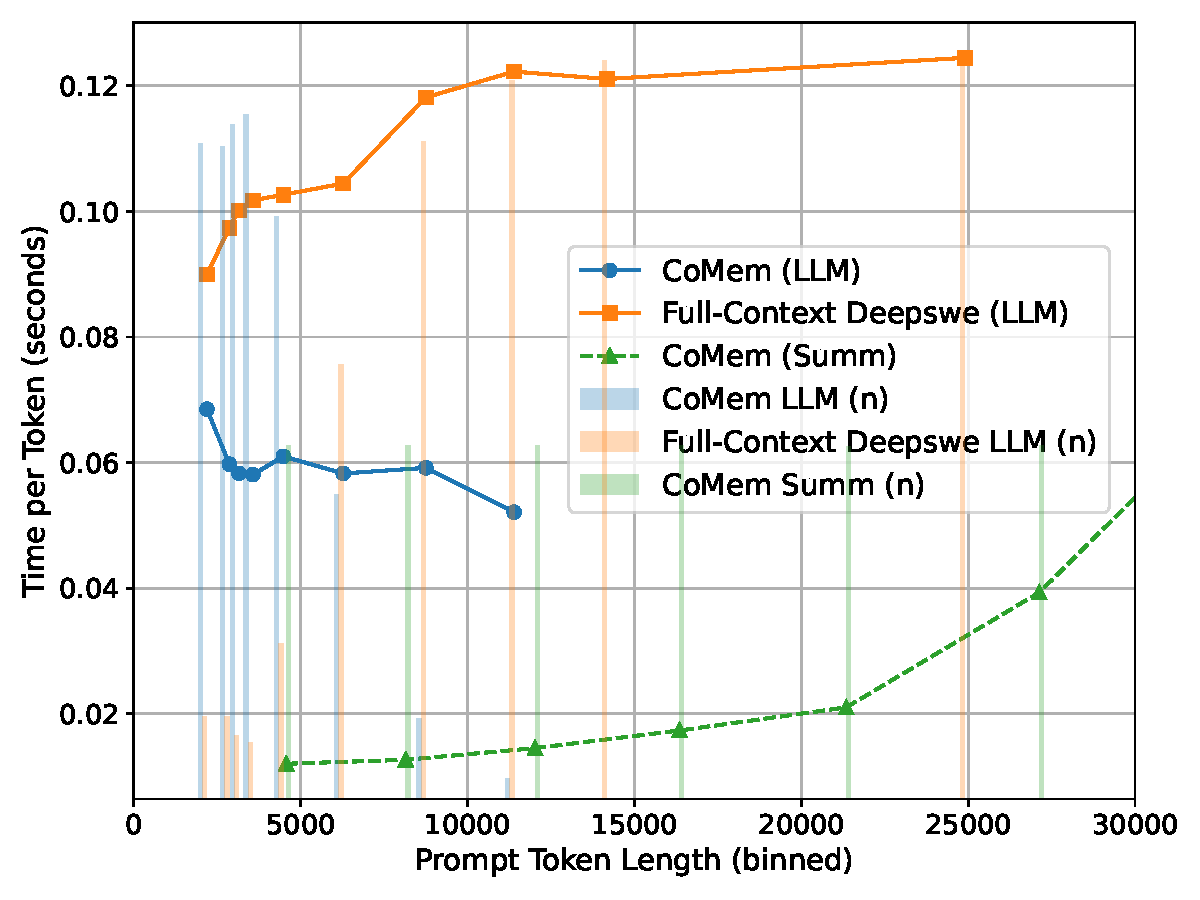
\includegraphics[width=\linewidth]{figs/time_per_token_by_prompt_length.pdf}
        % \caption{SciWorld}
        \label{fig:success-env3}
    \end{subfigure}
    \vspace{-5mm}
    \caption{
        Profiling results for agentic inference scenario. Left is the execution time for Full-Context baseline. Middle is the execution time for \model. Right is the time per completion token results.
    }
    \vspace{-5mm}
    \label{fig:agentic-profile}
\end{figure*}
In agentic inference, since at each step, only the current observations are prefilled, the total time is typically dominated by the decoding stage, which is often memory-bound because of the loading of KV cache. Thus, we study the decoding speed in this section in both synthetic long-context and standard agent inference scenarios.

\noindent \textbf{Long-context Scenario.} Real-time agentic inference often involves additional overheads from external processes such as I/O, as well as varying batch sizes and token lengths during rollout. To isolate the relationship between context length and decoding time, we first conduct a profiling analysis on a synthetic long-context scenario in which inputs and outputs are random data with fixed lengths and a constant batch size. As shown in Figure~\ref{fig:profile}, when the batch size is small (batch=$1$), TPOT does not scale significantly with context length, because the time spent loading the KV cache is negligible compared with other overheads such as loading model weights. For batch=$16$, at shorter contexts ($<2^{13}$), the KV cache remains small enough that GPU memory bandwidth is not saturated, and TPOT is still dominated by fixed overheads. Beyond $2^{13}$ tokens, however, the KV cache becomes large enough that each additional token incurs a linear increase in latency. For large batch sizes (batch=$64$), the GPU memory bandwidth is fully saturated even at short contexts, so TPOT scales linearly throughout.

\noindent \textbf{Agentic Scenario.} To further investigate how context-length-induced slow-down manifests during agentic inference, we measure the per-step execution time and its constituent components, averaged across multiple trajectories generated on SWE-Bench-Verified. The results are presented in the left panel of Figure~\ref{fig:agentic-profile}. We make two key observations. First, the total wall-clock time at each step is predominantly attributed to LLM execution, whereas environment execution constitutes a negligible fraction. Second, the LLM execution time exhibits a non-monotonic trend, increasing progressively from the initial steps up to approximately step 20, after which it begins to decrease toward the final steps.
% The explanation that in the beginning, the batch size is large and the decoding is still memory-bound, and later on, a few requests have been finished and then the batch size decreases which results in faster decoding.
We attribute this non-monotonic behavior to the evolving batch-size dynamics during inference. In the early stages, the large batch size renders the decoding process memory-bound, leading to increased latency as context lengths grow. As the generation progresses and individual requests reach completion, the effective batch size diminishes, thereby alleviating the memory bandwidth bottleneck and reducing per-step inference latency.
To disentangle the effect of prompt length from that of batch-size variation, we further present the execution time per completion token as a function of prompt length in the right panel of Figure~\ref{fig:agentic-profile} (orange line). The results demonstrate that decoding latency per token increases monotonically with prompt length, thereby corroborating the hypothesis that longer contexts incur proportionally greater decoding overhead.